\documentclass[conference]{IEEEtran}
\IEEEoverridecommandlockouts

\usepackage[utf8]{inputenc}
\usepackage[T1]{fontenc}
\usepackage[brazil]{babel}
\usepackage{amsmath,amssymb}
\usepackage{graphicx}
\usepackage{booktabs}
\usepackage{algorithm}
\usepackage{algorithmic}
\usepackage{url}
\usepackage{cite}

\renewcommand{\algorithmicrequire}{\textbf{Entrada:}}
\renewcommand{\algorithmicensure}{\textbf{Saída:}}
\renewcommand{\algorithmicfor}{\textbf{para}}
\renewcommand{\algorithmicdo}{\textbf{faça}}
\renewcommand{\algorithmicwhile}{\textbf{enquanto}}
\renewcommand{\algorithmicif}{\textbf{se}}
\renewcommand{\algorithmicthen}{\textbf{então}}
\renewcommand{\algorithmicend}{\textbf{fim}}
\renewcommand{\algorithmicreturn}{\textbf{retorne}}
\floatname{algorithm}{Algoritmo}

\begin{document}

\title{Análise de Centralidade em Redes Sociais:\\ Grau, \textit{Closeness} e \textit{Betweenness} na Rede ego-Facebook}

\author{\IEEEauthorblockN{João Marcelo França Batista}
\IEEEauthorblockA{Instituto de Ciência e Tecnologia (ICT) --- Universidade Federal de São Paulo (Unifesp)\\
São José dos Campos, SP, Brasil\\
joao.franca21@unifesp.br}}

\maketitle

\begin{abstract}
Este trabalho implementa, em linguagem C, a leitura de uma rede real em formato de lista de arestas e o cálculo de três medidas de centralidade para todos os seus vértices: grau, \textit{closeness} (proximidade) e \textit{betweenness} (intermediação). A base escolhida é a rede ego-Facebook do SNAP, com 4.039 vértices e 88.234 arestas. O grafo é armazenado em listas de adjacência, os identificadores são mapeados por uma tabela hash, as distâncias são obtidas por busca em largura (BFS) e o \textit{betweenness} é calculado pelo algoritmo de Brandes, em $O(VE)$. Os resultados foram conferidos com a biblioteca NetworkX, com erro máximo de $5\times10^{-11}$, e a implementação em C foi cerca de 37 vezes mais rápida. Em um notebook com processador Intel Core i5-1035G1, o \textit{closeness} levou 1,06\,s e o \textit{betweenness} 2,73\,s. O vértice 107 lidera as três medidas, e os vértices de maior intermediação são justamente os que ligam as comunidades da rede.
\end{abstract}

\begin{IEEEkeywords}
grafos, centralidade, betweenness, closeness, algoritmo de Brandes, busca em largura, redes sociais
\end{IEEEkeywords}

\section{Introdução}

Em teoria dos grafos e análise de redes complexas, as medidas de centralidade indicam quais vértices são mais importantes em um grafo. Elas são usadas para identificar as pessoas mais influentes de uma rede social, os elementos críticos de redes de infraestrutura (Internet, transporte, energia) e os principais espalhadores de uma epidemia~\cite{wasserman1994,freeman1978}.

Cada medida captura uma ideia diferente de importância. O \textbf{grau} conta as conexões diretas de um vértice. O \textbf{\textit{closeness}} mede o quão perto, em média, um vértice está de todos os outros~\cite{sabidussi1966}. O \textbf{\textit{betweenness}} mede quantas vezes um vértice aparece como ``ponte'' nos caminhos mínimos entre outros pares de vértices~\cite{freeman1977}.

O objetivo deste trabalho é implementar essas três medidas do zero, sem bibliotecas de grafos, aplicá-las a uma rede social real e analisar a corretude, o custo computacional e o que os resultados dizem sobre a rede. A Seção~\ref{sec:base} descreve a base de dados; a Seção~\ref{sec:metodo}, as estruturas de dados e os algoritmos; a Seção~\ref{sec:exp}, o ambiente e os tempos de execução; e a Seção~\ref{sec:res}, os resultados.

\section{Base de dados}\label{sec:base}

A base utilizada é a \textbf{ego-Facebook}, do repositório SNAP da Universidade Stanford~\cite{snap2014}. Ela foi coletada por McAuley e Leskovec~\cite{mcauley2012} a partir de usuários que responderam a uma pesquisa por meio de um aplicativo do Facebook. Cada vértice é um usuário (com identificador anonimizado) e cada aresta é uma amizade, de modo que o grafo é \textbf{não dirigido} e \textbf{não ponderado}. A rede é a união das redes de amigos (``redes ego'') de 10 usuários centrais, os \textit{egos}, que são os vértices 0, 107, 348, 414, 686, 698, 1684, 1912, 3437 e 3980.

O arquivo \texttt{facebook\_combined.txt} tem uma aresta ``$u$ $v$'' por linha. A Tabela~\ref{tab:base} resume as propriedades do grafo obtidas pelo programa. O diâmetro e o coeficiente de agrupamento foram calculados com o NetworkX~\cite{networkx2008}, apenas para caracterizar a rede.

\begin{table}[htbp]
\caption{Propriedades da rede ego-Facebook}
\label{tab:base}
\centering
\begin{tabular}{lr}
\toprule
Propriedade & Valor \\
\midrule
Vértices ($n$) & 4.039 \\
Arestas ($m$) & 88.234 \\
Densidade $2m/(n(n-1))$ & 1,082\% \\
Grau médio $2m/n$ & 43,69 \\
Grau mediano & 25 \\
Grau mínimo / máximo & 1 / 1.045 \\
Componentes conexas & 1 \\
Distância média entre pares & 3,69 \\
Diâmetro & 8 \\
Coeficiente de agrupamento médio & 0,606 \\
\bottomrule
\end{tabular}
\end{table}

A densidade de cerca de 1\% indica um grafo \textbf{esparso}, o que orientou a escolha da estrutura de dados. O grafo é conexo, então todos os pares de vértices têm distância finita. A distância média de 3,69 e o agrupamento alto são típicos de redes sociais de ``mundo pequeno''.

\section{Metodologia}\label{sec:metodo}

Todo o processamento foi implementado em C, em um único arquivo-fonte, com um menu que executa os itens pedidos no enunciado. O NetworkX foi usado apenas para desenhar o grafo e para conferir os resultados.

\subsection{Representação do grafo: lista $\times$ matriz de adjacência}

O grafo é armazenado em \textbf{listas de adjacência}~\cite{ziviani2011,cormen2012}: cada vértice tem um vetor dinâmico com seus vizinhos, que dobra de tamanho quando fica cheio. Como o grafo é não dirigido, cada aresta $\{u,v\}$ é guardada nas duas listas.

Uma matriz de adjacência teria $n^2 \approx 16{,}3$ milhões de células, das quais apenas 1,08\% seriam 1. Mesmo com 1 byte por célula, ela ocuparia 15,56\,MB, contra 0,67\,MB das listas ($2m$ inteiros de 4 bytes). O custo de tempo pesa ainda mais: para percorrer os vizinhos de um vértice, a matriz exige varrer uma linha inteira ($O(n)$), o que faz uma BFS custar $O(n^2)$ e o cálculo das métricas para todos os vértices custar $O(n^3) \approx 6{,}6\times10^{10}$ operações. Com listas, a BFS custa $O(n+m)$. A matriz só compensaria em grafos densos ou quando a consulta ``existe a aresta $(u,v)$?'' fosse a operação dominante.

\subsection{Leitura e mapeamento de identificadores}

Os identificadores do arquivo não precisam ser sequenciais. Por isso, uma \textbf{tabela hash} com endereçamento aberto e sondagem linear mapeia cada identificador original para um índice interno de 0 a $n-1$. A função hash usa o método da multiplicação, com a constante de Knuth $\lfloor 2^{64}/\phi \rfloor$~\cite{knuth1998,cormen2012}. O tamanho da tabela é uma potência de 2, e ela é duplicada (\textit{rehash}) quando o fator de carga passaria de 0,5. Na leitura, linhas iniciadas por \texttt{\#} ou \texttt{\%} são tratadas como comentários, e laços ($u=v$) e arestas repetidas são descartados. Na ego-Facebook não há nenhum dos dois.

\subsection{Grau}

O grau de $v$ é o tamanho da sua lista de adjacência, obtido em $O(1)$ por vértice e $O(n)$ no total. O programa também mostra o grau normalizado $d(v)/(n-1)$.

\subsection{Closeness}

Como as arestas não têm peso, uma \textbf{busca em largura} (BFS) a partir de $v$ visita os vértices em ordem crescente de distância e já fornece os caminhos mínimos $d(v,u)$ em $O(n+m)$~\cite{cormen2012}. Por isso não foi preciso usar Dijkstra, que só é necessário com pesos, nem Floyd--Warshall, que custaria $O(n^3)$. O enunciado define o \textit{closeness} como o comprimento médio dos caminhos mínimos de $v$ até os demais vértices, o que o programa imprime como ``distância média''. Nessa definição, quanto \emph{menor} o valor, mais central é o vértice. Para que o ranking tenha o sentido usual (maior $=$ mais central), usa-se o inverso~\cite{sabidussi1966}:
\begin{equation}
C_C(v) = \frac{r-1}{\sum_{u} d(v,u)} \cdot \frac{r-1}{n-1},
\end{equation}
em que $r$ é o número de vértices alcançáveis a partir de $v$ (incluindo ele). O segundo fator é a correção de Wasserman e Faust~\cite{wasserman1994} para grafos desconexos, a mesma adotada pelo NetworkX. Como a ego-Facebook é conexa ($r=n$), a expressão se reduz a $(n-1)/\sum_u d(v,u)$. Executando uma BFS por vértice, o custo total é $O(n(n+m))$.

\subsection{Betweenness: algoritmo de Brandes}

O \textit{betweenness} de $v$ é
\begin{equation}
C_B(v) = \sum_{s \neq v \neq t} \frac{\sigma_{st}(v)}{\sigma_{st}},
\end{equation}
em que $\sigma_{st}$ é o número de caminhos mínimos entre $s$ e $t$ e $\sigma_{st}(v)$ é quantos deles passam por $v$~\cite{freeman1977}. Calcular essa soma diretamente, como sugere a definição, exige enumerar caminhos para todos os $O(n^2)$ pares, com custo $O(n^3)$ ou pior. O algoritmo de Brandes~\cite{brandes2001} obtém o mesmo valor em $O(nm)$ para grafos não ponderados, usando a \emph{dependência} de $s$ em relação a $v$:
\begin{equation}
\delta_s(v) = \sum_{w:\, v \in P_s(w)} \frac{\sigma_{sv}}{\sigma_{sw}}\left(1 + \delta_s(w)\right),
\end{equation}
em que $P_s(w)$ é o conjunto de predecessores de $w$ nos caminhos mínimos que partem de $s$. Para cada origem $s$, uma BFS conta os caminhos mínimos $\sigma$. Em seguida, os vértices são percorridos do mais distante para o mais próximo, acumulando $\delta$ (Algoritmo~\ref{alg:brandes}). A própria fila da BFS, que guarda os vértices em ordem não decrescente de distância, é percorrida de trás para frente no lugar de uma pilha. Os predecessores não são armazenados: são os vizinhos $v$ de $w$ com $d(v)=d(w)-1$. Como cada par $\{s,t\}$ é contado nos dois sentidos, o resultado final é dividido por 2. O programa também mostra o valor normalizado por $(n-1)(n-2)/2$. Como $\sigma$ pode crescer exponencialmente, ele é armazenado em \texttt{double}.

\begin{algorithm}[htbp]
\caption{Brandes (grafo não dirigido e não ponderado)}
\label{alg:brandes}
\begin{algorithmic}[1]
\REQUIRE grafo $G=(V,E)$ em listas de adjacência
\ENSURE $C_B[v]$ para todo $v \in V$
\STATE $C_B[v] \leftarrow 0$ para todo $v$
\FOR{cada $s \in V$}
  \STATE $d[\cdot] \leftarrow -1$; $\sigma[\cdot] \leftarrow 0$; $\delta[\cdot] \leftarrow 0$
  \STATE $d[s] \leftarrow 0$; $\sigma[s] \leftarrow 1$; $Q \leftarrow [s]$
  \FOR{cada $v$ retirado de $Q$, em ordem}
    \FOR{cada vizinho $w$ de $v$}
      \IF{$d[w] < 0$}
        \STATE $d[w] \leftarrow d[v]+1$; insere $w$ no fim de $Q$
      \ENDIF
      \IF{$d[w] = d[v]+1$}
        \STATE $\sigma[w] \leftarrow \sigma[w] + \sigma[v]$
      \ENDIF
    \ENDFOR
  \ENDFOR
  \FOR{cada $w \neq s$ de $Q$, do último ao primeiro}
    \FOR{cada vizinho $v$ de $w$ com $d[v] = d[w]-1$}
      \STATE $\delta[v] \leftarrow \delta[v] + \frac{\sigma[v]}{\sigma[w]}(1+\delta[w])$
    \ENDFOR
    \STATE $C_B[w] \leftarrow C_B[w] + \delta[w]$
  \ENDFOR
\ENDFOR
\STATE $C_B[v] \leftarrow C_B[v]/2$ para todo $v$
\end{algorithmic}
\end{algorithm}

\subsection{Ordenação, busca e visualização}

Os rankings são ordenados por \textbf{merge sort} ($O(n \log n)$, estável), em ordem crescente, como pede o enunciado. Empates são desfeitos pelo identificador. A tela mostra os 15 primeiros e os 15 últimos vértices, além do top-10 do maior para o menor. A lista completa é gravada nos arquivos \texttt{ranking\_\allowbreak *.txt}.

A busca de um vértice usa a própria tabela hash ($O(1)$ em média). Para comparação, o programa mede também uma busca sequencial no vetor de identificadores ($O(n)$). A busca de uma aresta $(u,v)$ percorre a lista do extremo de menor grau e informa a distância entre $u$ e $v$ calculada pela BFS.

Para a visualização, o programa exporta o grafo e as métricas em CSV (formato também aceito pelo Gephi), e um script em Python desenha o grafo com NetworkX e matplotlib. As posições dos vértices são calculadas pelo algoritmo de Fruchterman--Reingold~\cite{fruchterman1991}. O tamanho de cada vértice é o seu \textit{betweenness} e a cor é o seu \textit{closeness}, ambos calculados pelo programa em C.

\section{Experimentos}\label{sec:exp}

\begin{figure*}[!t]
\centering
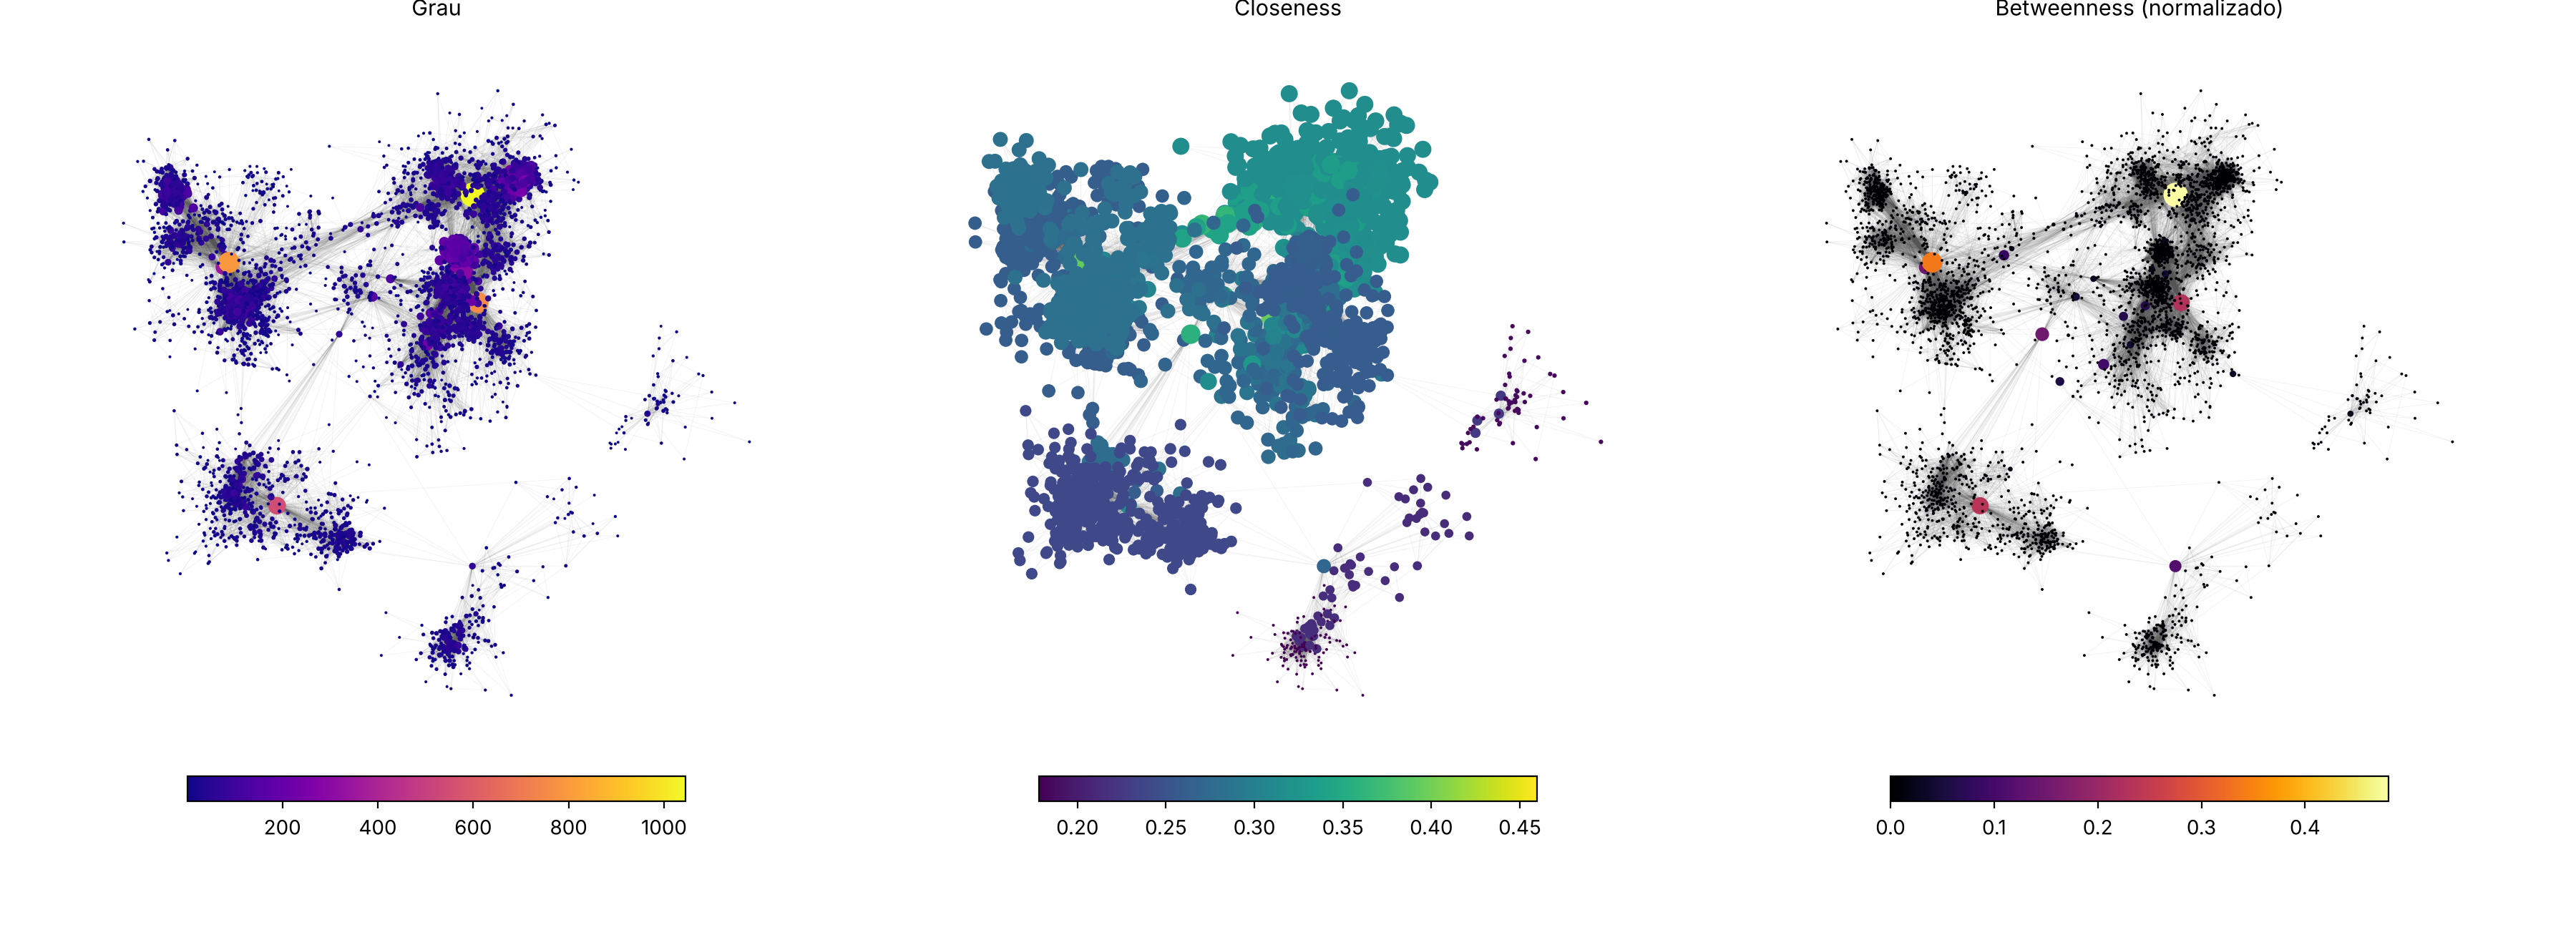
\includegraphics[width=\textwidth]{figuras/grafo_metricas.png}
\caption{Rede ego-Facebook, com o mesmo layout da Fig.~\ref{fig:grafo}, colorida por grau (esquerda), \textit{closeness} (centro) e \textit{betweenness} normalizado (direita). O tamanho do vértice acompanha a métrica de cada painel.}
\label{fig:metricas}
\end{figure*}

\subsection{Ambiente}

Os tempos principais foram medidos em um notebook ASUS VivoBook X515JF com processador Intel Core i5-1035G1 e 8\,GB de RAM, em uma máquina virtual Linux (Ubuntu 22.04, 2 vCPUs, 2,8\,GB de RAM, gcc 11.4.0). O programa foi compilado com \texttt{-O2} e com \texttt{-O0}. O tempo foi medido com \texttt{clock\_\allowbreak gettime}, e cada métrica foi executada 3 vezes. A comparação com o NetworkX 3.7 (Python 3.13) foi feita em outra máquina, um servidor Linux com processador Intel Xeon de 2,1\,GHz e gcc 13.3, onde os dois programas rodaram no mesmo ambiente.

\subsection{Tempos de execução}

A Tabela~\ref{tab:tempos} mostra os tempos médios no notebook. O grau e a ordenação são praticamente instantâneos. O custo está no \textit{closeness} e no \textit{betweenness}, que executam uma BFS para cada um dos 4.039 vértices. Cada BFS percorre $n + 2m \approx 1{,}8\times10^5$ posições, o que dá cerca de $7{,}3\times10^8$ passos para o \textit{closeness}. O algoritmo de Brandes percorre as listas duas vezes por origem (contagem e acumulação) e faz operações em ponto flutuante, o que explica por que leva cerca de 2,6 vezes mais que o \textit{closeness}. A otimização \texttt{-O2} reduziu os tempos em cerca de 3 vezes.

\begin{table}[htbp]
\caption{Tempo médio de 3 execuções no notebook (ego-Facebook)}
\label{tab:tempos}
\centering
\begin{tabular}{llrr}
\toprule
Etapa & Complexidade & \texttt{-O2} (s) & \texttt{-O0} (s) \\
\midrule
Leitura e construção & $O(n+m)$ & 0,012 & 0,026 \\
Grau & $O(n)$ & 0,00002 & 0,00003 \\
\textit{Closeness} & $O(n(n+m))$ & 1,060 & 3,283 \\
\textit{Betweenness} & $O(nm)$ & 2,726 & 8,797 \\
Ordenação & $O(n\log n)$ & 0,0008 & 0,0013 \\
\bottomrule
\end{tabular}
\end{table}

As variações entre as execuções foram pequenas: com \texttt{-O2}, o \textit{closeness} ficou entre 1,00 e 1,10\,s e o \textit{betweenness} entre 2,67 e 2,76\,s. No servidor, a versão em C levou 0,69\,s (\textit{closeness}) e 2,14\,s (\textit{betweenness}), contra 25,6\,s e 81,1\,s do NetworkX: cerca de 37 e 38 vezes mais rápida.

A busca também mostrou a diferença entre as estruturas. Na média de $10^6$ consultas, a tabela hash levou de 1,4 a 2,2\,ns por busca. A busca sequencial levou 38,6\,ns para o vértice 107, que está na posição 107 do vetor, e 1.440\,ns para um identificador inexistente (5000), que obriga a percorrer os 4.039 vértices.

\subsection{Validação}

Os três vetores de saída foram comparados com as funções \texttt{degree\_\allowbreak centrality}, \texttt{closeness\_\allowbreak centrality} e \texttt{betweenness\_\allowbreak centrality} do NetworkX~\cite{networkx2008}. O erro absoluto máximo foi de $5\times10^{-11}$ nas três métricas, o que corresponde apenas ao arredondamento das 10 casas decimais gravadas no CSV. O mesmo teste foi feito na rede do clube de karatê de Zachary~\cite{zachary1977} (34 vértices), em que o vértice 1 obteve \textit{betweenness} de 231,07 (0,4376 normalizado), o valor conhecido na literatura. Também foi testado um grafo sintético de 4.040 vértices com identificadores não sequenciais, um laço e uma aresta repetida.

\section{Resultados e discussão}\label{sec:res}

A Tabela~\ref{tab:top} mostra os 10 vértices de maior valor em cada métrica, e a Tabela~\ref{tab:bottom}, o início dos vetores em ordem crescente. Os vetores completos, com os 4.039 vértices, estão nos arquivos \texttt{ranking\_\allowbreak grau.txt}, \texttt{ranking\_\allowbreak closeness.txt} e \texttt{ranking\_\allowbreak betweenness.txt}.

\begin{table}[htbp]
\caption{Top-10 de cada métrica (vértice: valor)}
\label{tab:top}
\centering
\setlength{\tabcolsep}{4pt}
\begin{tabular}{r rr rr rr}
\toprule
& \multicolumn{2}{c}{Grau} & \multicolumn{2}{c}{\textit{Closeness}} & \multicolumn{2}{c}{\textit{Betw.} (norm.)} \\
\cmidrule(lr){2-3}\cmidrule(lr){4-5}\cmidrule(lr){6-7}
\# & $v$ & $d(v)$ & $v$ & $C_C$ & $v$ & $C_B$ \\
\midrule
1 & 107 & 1045 & 107 & 0,4597 & 107 & 0,4805 \\
2 & 1684 & 792 & 58 & 0,3974 & 1684 & 0,3378 \\
3 & 1912 & 755 & 428 & 0,3948 & 3437 & 0,2361 \\
4 & 3437 & 547 & 563 & 0,3939 & 1912 & 0,2293 \\
5 & 0 & 347 & 1684 & 0,3936 & 1085 & 0,1490 \\
6 & 2543 & 294 & 171 & 0,3705 & 0 & 0,1463 \\
7 & 2347 & 291 & 348 & 0,3699 & 698 & 0,1153 \\
8 & 1888 & 254 & 483 & 0,3698 & 567 & 0,0963 \\
9 & 1800 & 245 & 414 & 0,3695 & 58 & 0,0844 \\
10 & 1663 & 235 & 376 & 0,3666 & 428 & 0,0643 \\
\bottomrule
\end{tabular}
\end{table}

\begin{table}[htbp]
\caption{Início dos vetores em ordem crescente}
\label{tab:bottom}
\centering
\setlength{\tabcolsep}{4pt}
\begin{tabular}{r rr rr rr}
\toprule
& \multicolumn{2}{c}{Grau} & \multicolumn{2}{c}{\textit{Closeness}} & \multicolumn{2}{c}{\textit{Betweenness}} \\
\cmidrule(lr){2-3}\cmidrule(lr){4-5}\cmidrule(lr){6-7}
\# & $v$ & $d(v)$ & $v$ & $C_C$ & $v$ & $C_B$ \\
\midrule
1 & 11 & 1 & 692 & 0,17825 & 11 & 0 \\
2 & 12 & 1 & 801 & 0,17825 & 12 & 0 \\
3 & 15 & 1 & 699 & 0,17826 & 15 & 0 \\
4 & 18 & 1 & 744 & 0,17826 & 18 & 0 \\
5 & 37 & 1 & 749 & 0,17826 & 32 & 0 \\
\bottomrule
\end{tabular}
\end{table}

\begin{figure}[!t]
\centering
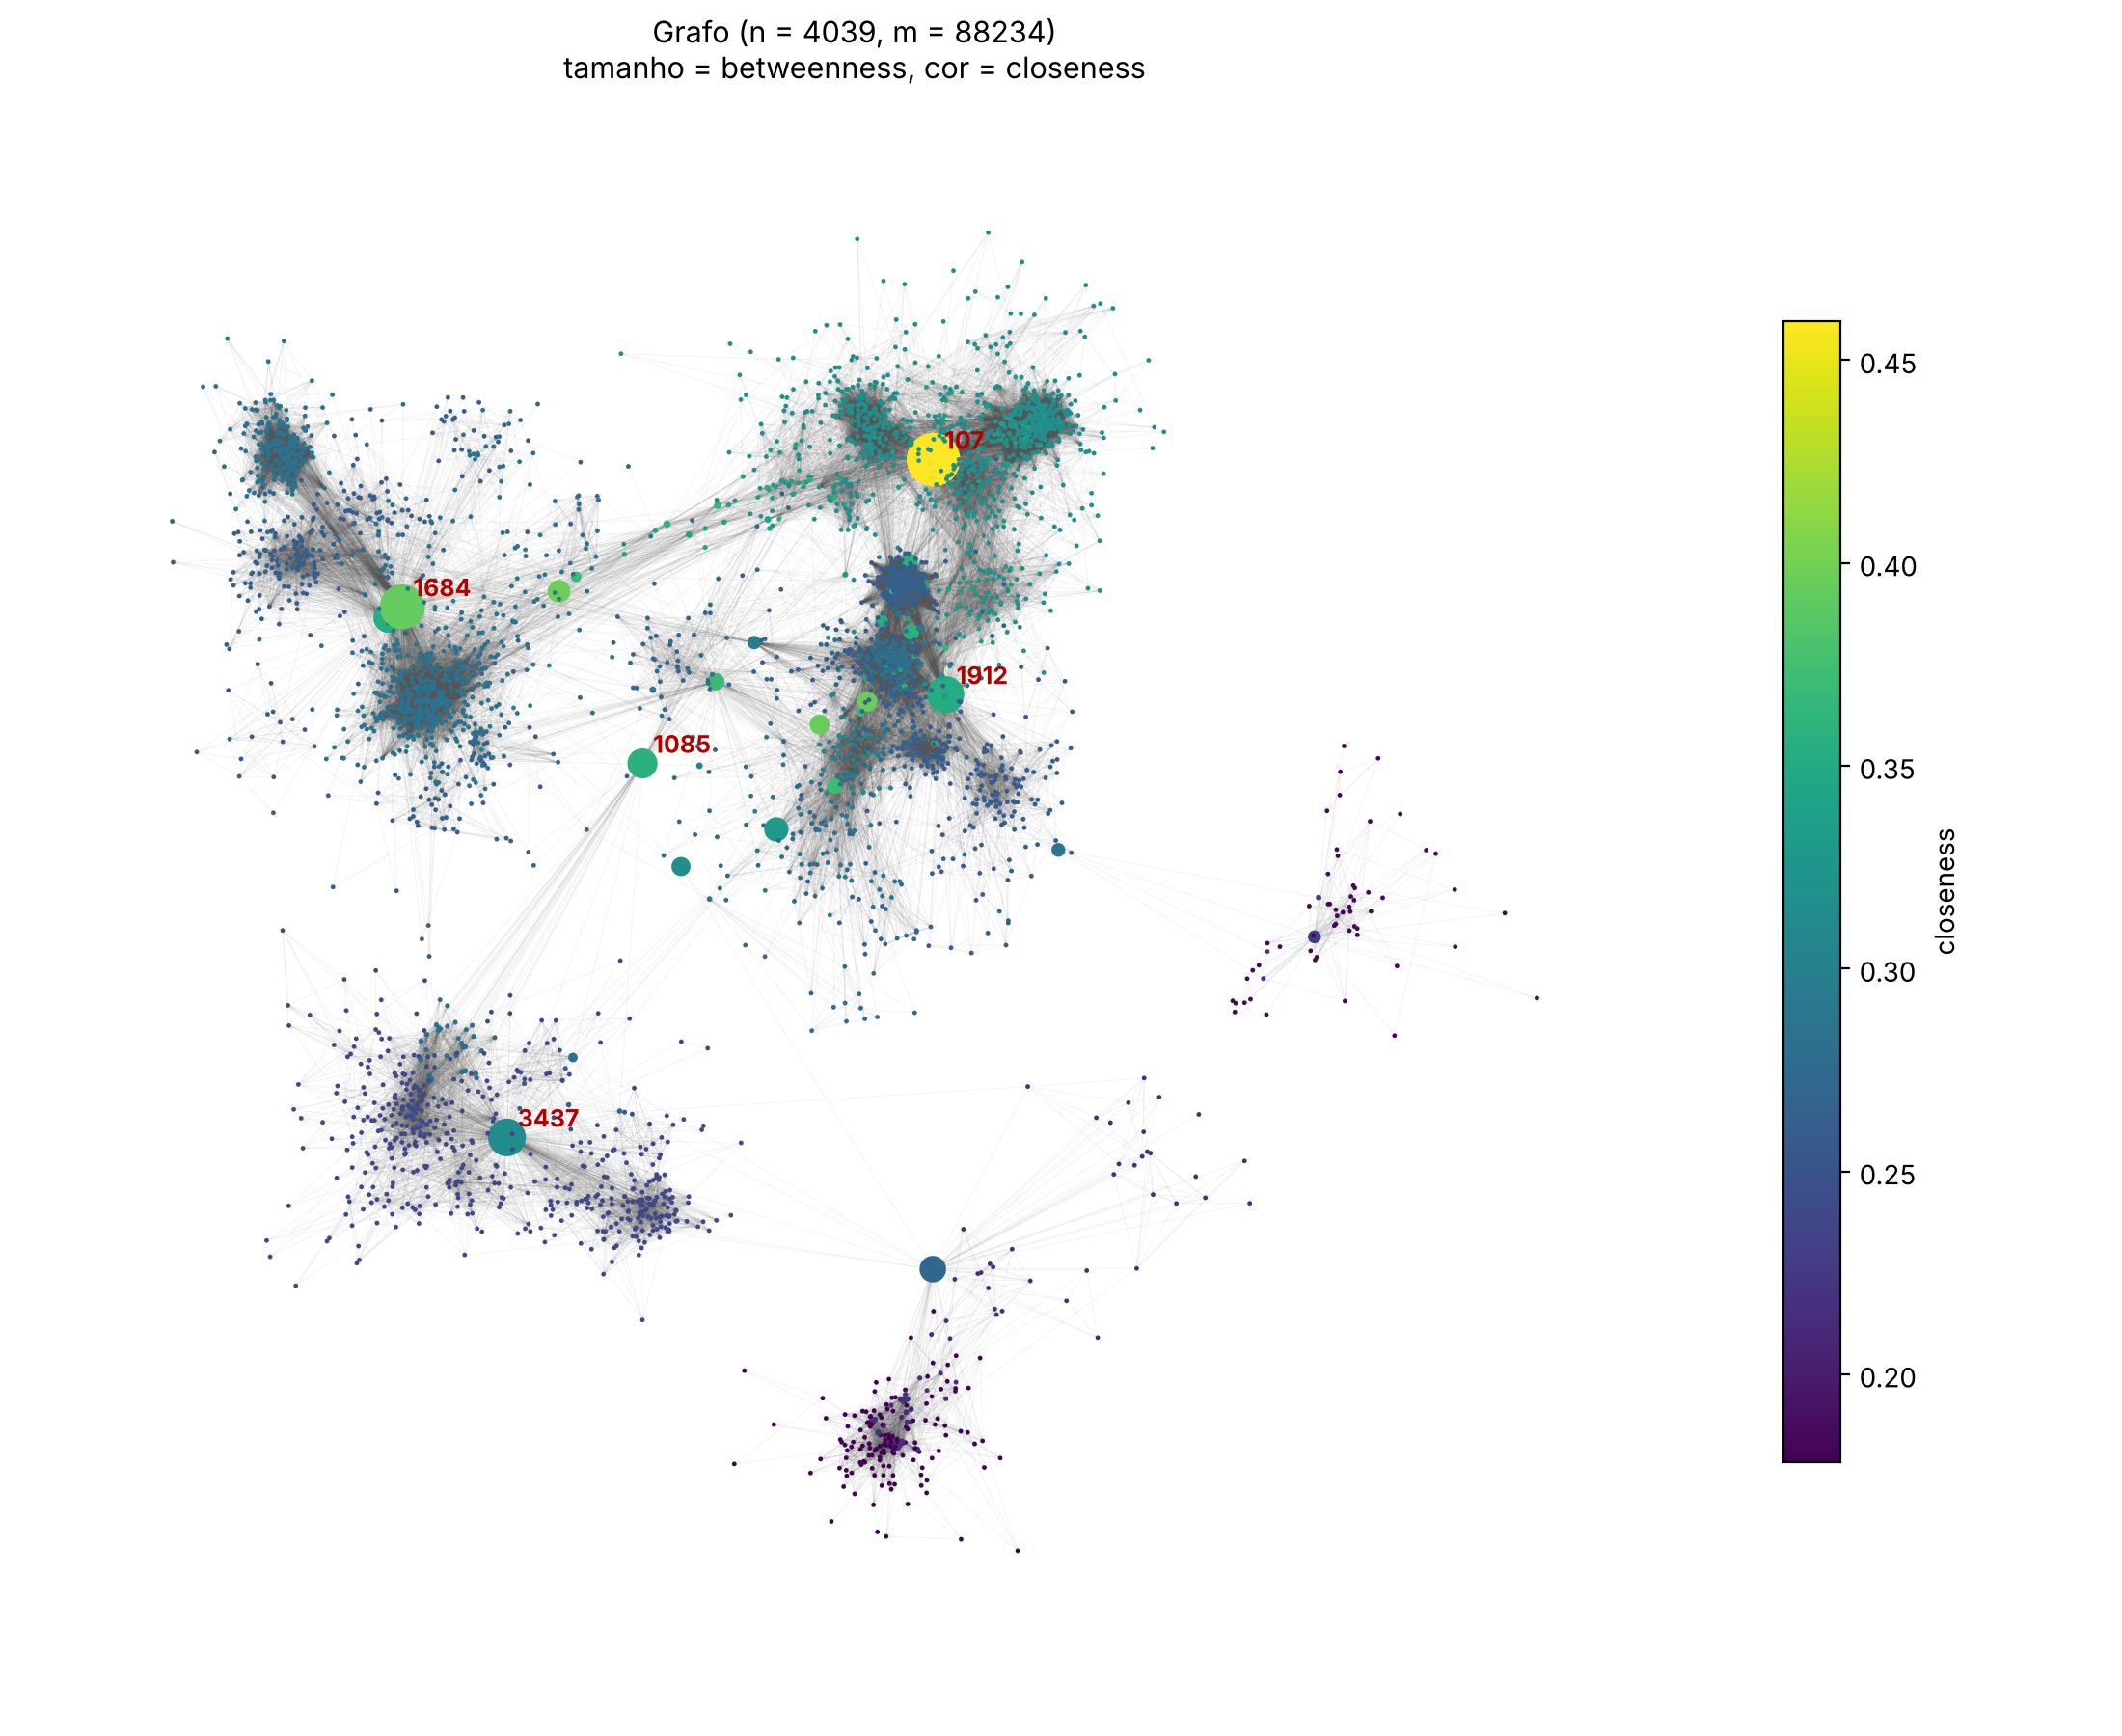
\includegraphics[width=\columnwidth]{figuras/grafo_plot.png}
\caption{Rede ego-Facebook desenhada com Fruchterman--Reingold. Tamanho do vértice $=$ \textit{betweenness}, cor $=$ \textit{closeness}. Em vermelho, os 5 vértices de maior \textit{betweenness}.}
\label{fig:grafo}
\end{figure}


\textbf{O vértice 107 lidera as três métricas.} Ele tem 1.045 amigos (25,9\% da rede), a menor distância média até os demais (2,18 passos) e \textit{betweenness} normalizado de 0,48: em média, quase metade dos caminhos mínimos entre pares de outros vértices passa por ele. Sozinho, ele concentra 17,8\% da soma de todos os valores de \textit{betweenness}.

\textbf{O \textit{betweenness} é muito concentrado.} Os 10 primeiros vértices somam 72,0\% do total, enquanto 342 vértices (8,5\%) têm \textit{betweenness} zero: nenhum caminho mínimo entre outros dois vértices passa por eles. Isso inclui os 75 vértices de grau 1, que nunca podem servir de ponte. Na Fig.~\ref{fig:grafo}, os vértices grandes ficam exatamente nos pontos de ligação entre as comunidades. Seis dos 10 primeiros em \textit{betweenness} (107, 1684, 3437, 1912, 0 e 698) são egos da coleta, e todos os 10 egos estão entre os 20 primeiros. Isso é esperado, porque cada ego é o ponto de ligação de toda a sua rede de amigos.

\textbf{As métricas medem coisas diferentes.} A correlação de Spearman entre grau e \textit{betweenness} é alta (0,79), mas a do \textit{closeness} com as outras duas é moderada: 0,43 com o grau e 0,48 com o \textit{betweenness}. O caso mais claro é o vértice 58. Ele tem apenas 12 vizinhos (é o 2.918.º em grau), mas é o 2.º em \textit{closeness} e o 9.º em \textit{betweenness}, porque está ligado diretamente a quatro dos maiores \textit{hubs} da rede: 0, 107, 1684 e 1912. Outro exemplo é o vértice 1085, 5.º em \textit{betweenness} com 66 vizinhos (851.º em grau). Seus vizinhos se dividem entre a comunidade do vértice 107 e a do vértice 3437, das quais ele é uma das poucas ligações diretas. No outro extremo, os menores valores de \textit{closeness} (cerca de 0,178, ou seja, distância média de 5,6) estão nas comunidades periféricas, ligadas ao resto da rede por poucos vértices (Fig.~\ref{fig:metricas}).

Em uma rede social, esses perfis têm interpretações distintas. O grau indica popularidade local. O \textit{closeness} indica quem consegue fazer uma informação chegar mais rápido a toda a rede. O \textit{betweenness} indica quem controla o fluxo entre grupos. No caso do vértice 107, quase metade dos caminhos mínimos entre os outros pares passa por ele.

\section{Conclusão}

O trabalho implementou em C a leitura de uma rede real e o cálculo de grau, \textit{closeness} e \textit{betweenness} para todos os vértices. Os resultados coincidiram com os do NetworkX até o arredondamento, e a implementação foi cerca de 37 vezes mais rápida. As escolhas de estrutura de dados foram decisivas: as listas de adjacência mantêm a BFS em $O(n+m)$ em um grafo com 1\% de densidade, e o algoritmo de Brandes evita o custo cúbico da definição direta do \textit{betweenness}. Na ego-Facebook, as três métricas apontam o vértice 107 como o mais central. O \textit{betweenness} é bastante concentrado nos vértices que ligam comunidades, como os egos da coleta. Como trabalhos futuros, seria possível paralelizar as BFS, que são independentes entre si, e usar aproximações do \textit{betweenness} por amostragem de origens em redes maiores.

\section*{Nota sobre o uso de IA}

Uma LLM (Claude, da Anthropic) foi usada como apoio na implementação e nos comentários do código, na validação com o NetworkX, na geração das figuras e na redação deste relatório. Todos os resultados apresentados foram obtidos executando o programa.

\begin{thebibliography}{00}
\bibitem{freeman1977} L.~C. Freeman, ``A set of measures of centrality based on betweenness,'' \textit{Sociometry}, vol.~40, no.~1, pp.~35--41, 1977.
\bibitem{freeman1978} L.~C. Freeman, ``Centrality in social networks: conceptual clarification,'' \textit{Social Networks}, vol.~1, no.~3, pp.~215--239, 1978.
\bibitem{sabidussi1966} G. Sabidussi, ``The centrality index of a graph,'' \textit{Psychometrika}, vol.~31, no.~4, pp.~581--603, 1966.
\bibitem{brandes2001} U. Brandes, ``A faster algorithm for betweenness centrality,'' \textit{Journal of Mathematical Sociology}, vol.~25, no.~2, pp.~163--177, 2001.
\bibitem{wasserman1994} S. Wasserman e K. Faust, \textit{Social Network Analysis: Methods and Applications}. Cambridge: Cambridge University Press, 1994.
\bibitem{cormen2012} T.~H. Cormen, C.~E. Leiserson, R.~L. Rivest e C. Stein, \textit{Algoritmos: Teoria e Prática}, 3.~ed. Rio de Janeiro: Elsevier, 2012.
\bibitem{ziviani2011} N. Ziviani, \textit{Projeto de Algoritmos com Implementações em Pascal e C}, 3.~ed. São Paulo: Cengage Learning, 2011.
\bibitem{knuth1998} D.~E. Knuth, \textit{The Art of Computer Programming, Vol. 3: Sorting and Searching}, 2.~ed. Reading: Addison-Wesley, 1998.
\bibitem{mcauley2012} J. McAuley e J. Leskovec, ``Learning to discover social circles in ego networks,'' em \textit{Advances in Neural Information Processing Systems (NIPS)}, 2012.
\bibitem{snap2014} J. Leskovec e A. Krevl, ``SNAP Datasets: Stanford Large Network Dataset Collection,'' 2014. [Online]. Disponível: \url{https://snap.stanford.edu/data}
\bibitem{networkx2008} A.~A. Hagberg, D.~A. Schult e P.~J. Swart, ``Exploring network structure, dynamics, and function using NetworkX,'' em \textit{Proc. 7th Python in Science Conference (SciPy)}, 2008, pp.~11--15.
\bibitem{fruchterman1991} T.~M.~J. Fruchterman e E.~M. Reingold, ``Graph drawing by force-directed placement,'' \textit{Software: Practice and Experience}, vol.~21, no.~11, pp.~1129--1164, 1991.
\bibitem{zachary1977} W.~W. Zachary, ``An information flow model for conflict and fission in small groups,'' \textit{Journal of Anthropological Research}, vol.~33, no.~4, pp.~452--473, 1977.
\end{thebibliography}

\end{document}
